\chapter{Équations de bilan du laser et du mécanisme de pompe}
\section{Équation de bilan du laser et équations de Maxwell-Bloch}
Reprenons les équations de Maxwell-Bloch d'un laser
\begin{equation}
\left\{\begin{array}{lll}
\dot {\cal E}(t) &\DS=  - \frac{{{K_c}}}{2}{\cal E} + \frac{{i{\omega _c}}}{{2{\varepsilon _0}}}{\cal P}&\qquad(1)\vspace{2mm}\\
\dot {\cal P}(t) &\DS=  - {\gamma _ \bot }{\cal P} - \frac{i}{\hbar }|{\mu _{21}}{|^2}{\cal D}{\cal E} - i({\omega _a} - {\omega _c}){\cal P}(t)&\qquad(2)\vspace{2mm}\\
\dot {\cal D}(t) &\DS=  - {\gamma _\parallel }({{\cal D}} - {\hat {\cal D}}) - \frac{i}{{2\hbar }}({\cal P}{{\cal E}^*} - {\cal E}{{\cal P}^*})&\qquad(3)
\end{array}\right.
\end{equation}
Les différents temps de vies définissent les \textit{classes} des lasers : $AB$ si la polarisation 
est la plus rapide alors que si le champ est le plus lent, on parlera de la classe $A$. Faisons ici 
l'hypothèse que la polarisation répond très rapidement par rapport à la dynamique de $\mathcal{E}$ 
et $\mathcal{D}$
\begin{equation}
{\gamma _ \bot } \gg {\gamma _\parallel },{K_c}/2
\end{equation}
Considérons $\omega_a=\omega_c$ mais aussi $\omega_L=\omega_c$. La seconde équation de MB (2) devient
\begin{equation}
\dot {\cal P}(t) =  - {\gamma _ \bot }{\cal P} - \frac{i}{\hbar }|{\mu _{21}}{|^2}{\cal D}{\cal E}
\end{equation}
En supposant $\mathcal{E}, \mathcal{D}$ constant
\begin{equation}
{\cal P}(t) = {\cal P}(0){{\rm{e}}^{ - {\gamma _ \bot }t}} - \frac{{i|{\mu _{21}}{|^2}}}{{\hbar {\gamma _ \bot }}}{\cal E}{\cal D}(1 - {{\rm{e}}^{ - {\gamma _ \bot }t}})
\end{equation}
Si $t\gg 1/\gamma$ (équivalent à $\dot{\mathcal{P}}(t)=0$ dans (2)) 
\begin{equation}
{\cal P} =  - \frac{{i|{\mu _{21}}{|^2}}}{{\hbar {\gamma _ \bot }}}{\cal E}{\cal D}
\end{equation}
Il s'agit d'une évolution adiabatique de $\mathcal{P}$ qui garde sa valeurs stationnaire. Remplaçons 
cette dernière expression de $\mathcal{P}$ dans (1)
\begin{equation}
\dot {\cal E}(t) =  - \frac{{{K_c}}}{2}{\cal E} + \frac{{i{\omega _c}}}{{2{\varepsilon _0}}}\left( { - \frac{{i|{\mu _{21}}{|^2}}}{{\hbar {\gamma _ \bot }}}{\cal E}{\cal D}} \right)
\end{equation}
Faisons pareil avec (3)
\begin{equation}
\dot {\cal D}(t) =  - {\gamma _\parallel }({{\cal D}} - {\hat {\cal D}}) - \frac{{|{\mu _{21}}{|^2}}}{{2{\hbar ^2}{\gamma _ \bot }}}2{\cal D}|{\cal E}{|^2}
\end{equation}
Cette expression de l'inversion de population dépend du terme de pompage ainsi que du module carré 
de $\mathcal{E}$. Afin de remplacer l'une dans l'autre, on va multiplier cette expression par son 
conjugué ($\mathcal{E}^*\mathcal{E}=|\mathcal{E}|^2$). Si $\mathcal{I}=|\mathcal{E}|^2$, alors\\

\retenir{
\begin{equation}
\left\{\begin{array}{lll}
{\dot {\cal I}}(t) &\DS=  - {K_c}{{\cal I}} + \frac{{{\omega _c}|{\mu _{21}}{|^2}}}{{\hbar {\gamma _ \bot }{\varepsilon _0}}}{\cal D}{{\cal I}}&\qquad(4)\vspace{2mm}\\
\dot {\cal D}(t) &\DS=  - {\gamma _\parallel }({{\cal D}} - {\hat {\cal D}}) - \frac{{|{\mu _{21}}{|^2}}}{{{\hbar ^2}{\gamma _ \bot }}}{\cal D}{{\cal I}}&\qquad(5)
\end{array}\right.
\end{equation}
Ces deux équations sont connues comme les équations de bilan d'un laser. Elles décrivent la 
dynamique des laser de classes dynamiques $A$ et $B$.}


\section{Systèmes à deux niveaux}
	\begin{wrapfigure}[6]{r}{6cm}
	\vspace{-8mm}
	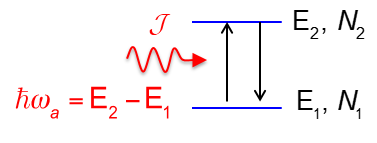
\includegraphics[scale=0.6]{ch4/image1.png}
	\captionof{figure}{ }
	\end{wrapfigure}
Considérons un flux de photon incident dont l'énergie est celle entre deux niveaux. Pour une onde 
monochromatique incidente à $\omega_0$ :
\begin{equation}
u = {n_p}\hbar {\omega _0}\delta (\omega  - {\omega _0}),\qquad 
{{\cal J}} = {n_p}{v_g},\qquad \hbar\omega_a = E_2-E_1
\end{equation}
Il est possible de calculer le taux d'absorption $\DS{\Gamma _{12}} = \int {{B_{12}}u(\omega )g(\omega ){N_1}{\rm{d}}\omega }$ en y remplaçant $u$ monochromatique 
\begin{equation}
{\Gamma _{12}} = \sigma {{\cal J}}{N_1}
\end{equation}
où $\DS \sigma  = B\hbar {\omega _0}g({\omega _0})/{v_g}$ est la section efficace ($m^2$). Le taux 
de variation de la population atomique s'exprime
\begin{equation}
{\dot N_2} = {\Gamma _{12}} - {\Gamma _{21}} - {T_{21}}{N_2},\qquad
{\dot N_1} =  - ({\Gamma _{12}} - {\Gamma _{21}}) + {T_{21}}{N_2}
\end{equation}
où ${T_{21}} = {A_{21}} + {S_{21}}$ (le premier est radiatif, pas le second)\footnote{Qu'est ce que 
ça représente exactement?}. En en tire
\begin{equation}
\frac{{\rm{d}}}{{{\rm{d}}t}}({N_1} + {N_2}) = 0 \Rightarrow {N_1} + {N_2} = N
\end{equation}
Pour la solution stationnaire (par exemple $\dot{N_2}=0$)
\begin{equation}
\sigma {{\cal J}}({N_1} - {N_2}) = {T_{21}}{N_2}
\end{equation}
Sachant que $\mathcal{D}=N_2-N_1\leftrightarrow \mathcal{D}+N=2N_2$ 
\begin{equation}
 - \sigma {{\cal J}{\cal D}} = {T_{21}}({{\cal D}} + N)/2\qquad\Rightarrow\qquad
{{\cal D}} =  - N\frac{1}{{1 + 2\sigma {{\cal J}}/{T_{21}}}}
\end{equation}
Cette expression est logique car s'il n 'y a pas de courant on trouve $\mathcal{D}=-N$ : on ne peut 
pas avoir d'inversion de population car $\mathcal{D}$ est toujours négatif.\\

Explicitons cette expression de l'inversion de population. Nous savons (en substituant les expressions 
terme à terme) que
\begin{equation}
2\sigma {{\cal J}}/{T_{21}} = 2\frac{{B\hbar {\omega _0}g({\omega _0})}}{{{v_g}}}\frac{I}{{\hbar {\omega _0}}}/{T_{21}} = \frac{I}{{{I_s}}}\tilde g({\omega _0})
\end{equation}
où $\tilde g({\omega _0}) = \frac{{g({\omega _0})}}{{g({\omega _a})}}$. L'\textbf{intensité de 
saturation} est définie comme ($W.m^{-2}$)
\begin{equation}
{I_s} = \frac{{{v_g}{T_{21}}}}{{2Bg({\omega _a})}}
\end{equation}
On arrive alors à ré-écrire $\mathcal{D}$
\begin{equation}
{{\cal D}} =  - N/[1 + \frac{I}{{{I_s}}}\tilde g({\omega _0})]
\end{equation}
Comme $\mathcal{D}<0$, cela montre qu'il n'est pas possible d'atteindre l'inversion de population 
dans un régime stationnaire ($\alpha = -\sigma\mathcal{D} > 0$, pas de gain). 
\begin{center}
	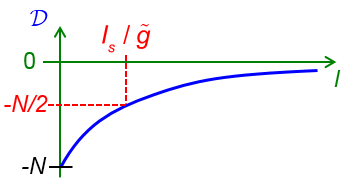
\includegraphics[scale=0.6]{ch4/image2.png}
	\captionof{figure}{ }
\end{center}
Considérons le cas 
d'une absorption
\begin{equation}
\frac{{\rm{d}}}{{{\rm{d}}z}}I =  - \alpha I
\end{equation}
où $\DS\alpha  =  - \sigma {{\cal D}} = \sigma N/[1 + \frac{I}{{{I_s}}}\tilde g({\omega _0})]$. 
Passons en revue deux cas 
\begin{enumerate}
\item $I\ll I_s$ (absorption non saturée)
\begin{equation}
\alpha\approx \sigma N \qquad \Rightarrow\qquad I(z) = {I_0}{\rm{exp(}} - \sigma Nz{\rm{)}}
\end{equation}
A faible intensité (par rapport à celle de saturation) il y a donc beaucoup d'absorption
\begin{center}
	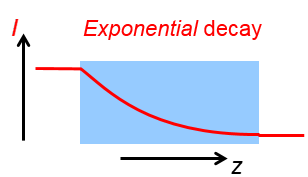
\includegraphics[scale=0.6]{ch4/image3.png}
	\captionof{figure}{ }
\end{center}


\item $I \gg I_s$ (absorption saturée)
\begin{equation}
\alpha  \approx \sigma N\frac{{{I_s}}}{I}\qquad\Rightarrow\qquad 
I(z) = {I_0} - {I_s}\sigma Nz
\end{equation}
Lorsque l'on atteint une intensité proche de celle de saturation, on observe une décroissance 
linéaire de l'intensité ce qui est une grosse différence. On parle de \textit{transparence 
auto-induite}\footnote{Heu..?}
\begin{center}
	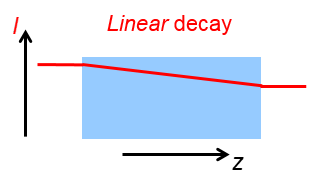
\includegraphics[scale=0.6]{ch4/image4.png}
	\captionof{figure}{ }
\end{center}
\end{enumerate}

Même si ce système a deux niveau, il n'est pas utile pour en faire un laser (car $\mathcal{D}<0$) 
mais on peut l'utiliser pour générer de courtes impulsions. Pour avoir un gain dans le système 
($\mathcal{D}>0$) il faut un système atomique avec plus de deux niveaux (au moins 
trois ou autre niveaux d'énergie participant au lasage/pomapge).

\section{Laser à trois niveaux d'énergie}
	\begin{wrapfigure}[7]{l}{6cm}
	\vspace{-5mm}
	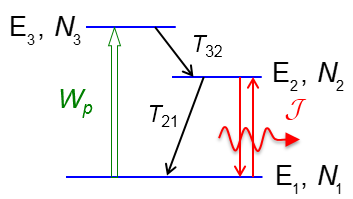
\includegraphics[scale=0.6]{ch4/image5.png}
	\captionof{figure}{ }
	\end{wrapfigure}
Pour contrer ce problème, nous allons utiliser un niveau de plus haute énergie dont le but est de 
nourrir le second niveau et non pas que deux niveau qui se peuplent et dépeuplent. L'idée est de 
s'arranger pour que le taux de $3\to1 \ll 3\to 2$. Nous allons ici considérer un système Er (erbium) 
à trois niveaux. La densité totale est la somme des densités de chaque niveau.
\begin{equation}
N= N_1+N_2+N_3\qquad (6)
\end{equation}
Comme annoncé, on fait l'hypothèse que le niveau 3 se désexcite préférentiellement vers le second 
niveau et non pas le fondamental
\begin{equation}
T_{31}N_3 \ll T_{32}N_3
\end{equation}
Soit $W_p=\sigma_p\mathcal{J}_p$ ($s^{-1}$) le taux de pompage optique. Étudions la variation de 
densité du niveau trois
\begin{equation}
{\dot N_3} = {W_p}{N_1} - {W_p}{N_3} - {T_{32}}{N_3}\qquad(7)
\end{equation}
Il s'agit de la contribution de la pompe, mais aussi l'émission stimulée $3\to1$ du à la pompe et 
aux transitions\footnote{Expliciter}. De même pour le niveau 2
\begin{equation}
{\dot N_2} =  + {T_{32}}{N_3} - ({N_2} - {N_1})\sigma {{\cal J}} - {T_{21}}{N_2}
\end{equation}
Il peut être peuplé depuis le niveau 3, il peut avoir de l'émission stimulée, de l'absorption et 
$T_{21}N_1$ l'émission stimulée de $2\to1$. En faisant de même pour le niveau fondamental
\begin{equation}
{\dot N_1} = ({N_2} - {N_1})\sigma {{\cal J}} + {T_{21}}{N_2} - {W_p}({N_1} - {N_3})
\end{equation}
En faisant un peu de mathématiques (non détaillées ici) on peut obtenir une équation donnant le 
rapport entre l'inversion de population et la densité totale
\begin{equation}
\frac{{{\cal D}}}{N} = \frac{{{W_p}({T_{32}} - {T_{21}}) - {T_{21}}{T_{32}}}}{{3\sigma {{\cal J}}{W_p} + 2{W_p}{T_{21}} + 2\sigma {{\cal J}}{T_{32}} + {T_{21}}{T_{32}} + {W_p}{T_{32}}}}
\end{equation}
Le dénominateur n'a que des signes positif. S'il n'y a pas de pompe, le rapport est négatif et on 
n'a pas d'inversion de population (ce qui est cohérent). Pour avoir une inversion, il faut que $T_{32}
\gg T_{21}$ ce qui signifie que le temps de désexcitation de $2\to3$ doit être plus petit que 
$2\to1$.\\

On peut définir un taux de pompage de transparence (autant d'absorption que d'émission stimulée, dès 
qu'un photon descend dans le niveau 1, un autre remonte directement dans le niveau 3). 
\begin{equation}
W_p^{t - th} = {T_{21}}{T_{32}}/({T_{32}} - {T_{21}})
\end{equation}
Pour obtenir ce milieu transparent, il faut que $T_{32}\gg T_{21} \Rightarrow W_p^{t - th} \approx {T_{21}}$. \\

Faisons cette supposition de milieu transparent impliquant une élimination adiabatique en $N_3$. Après 
quelques substitutions (slide 8)
\begin{equation}
{\dot {\cal D}} = 2{W_p}(N - {{\cal D}})/2 - 2{{\cal D}}\sigma {{\cal J}} - 2{T_{21}}(N + {{\cal D}})/2 =  - ({W_p} + {T_{21}}){{\cal D}} - 2{{\cal D}}\sigma {{\cal J}} + ({W_p} - {T_{21}})N
\end{equation}
La dernière égalité est formellement égale à
\begin{equation}
\dot {\cal D}(t) =  - {\gamma _\parallel }({{\cal D}} - {\hat {\cal D}}) - \frac{{|{\mu _{21}}{|^2}}}{{{\hbar ^2}{\gamma _ \bot }}}{\cal D}{{\cal I}}
\end{equation}

	\begin{wrapfigure}[9]{l}{6cm}
	\vspace{-12mm}
	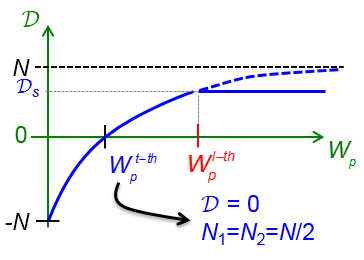
\includegraphics[scale=0.6]{ch4/image6.png}
	\captionof{figure}{ }
	\end{wrapfigure}
On trouve une valeur du coefficient de relaxation qui dépend de $T_{21}$ mais aussi du taux de 
pompage ce qui peut ne pas paraître évident. Tout se réparti donc entre le niveau fondamental et le 
second niveau, le niveau 3 n'est qu'une "étape nécessaire" pour atteindre le second niveau.\\

Regardons la solution stationnaire au dessus, en dessous et au seuil laser\\

\begin{itemize}
\item[$\bullet$] En dessous du seuil laser $\mathcal{J}=0$
\begin{equation}
{{\cal D}} = \frac{{({W_p} - {T_{21}})}}{{({W_p} + {T_{21}})}}N = {\hat {\cal D}}
\end{equation}
Lorsque $W_p > W_p^{t-th}, \mathcal{G}=\sigma\mathcal{D}$ et l'on retrouve un amplification 
exponentielle.
\item[$\bullet$] Au seuil laser.
\begin{equation}
{{{\cal G}}_s} = \sigma {{{\cal D}}_s} = {K_c}/c\qquad\Rightarrow\qquad 
W_p^{l - th} = {T_{21}}\frac{{1 + {K_c}/Nc\sigma }}{{1 - {K_c}/Nc\sigma }} > {T_{21}} = W_p^{t - th}
\end{equation}
On observe une diminution de la transparence $W$ si $T_{21}$ et $K_c$ diminuent.
\item[$\bullet$] Au dessus du seuil laser : $\mathcal{J}\neq0$
\begin{equation}
{{\cal D}} = \frac{{({W_p} - {T_{21}})/({W_p} + {T_{21}})}}{{1 + 2\sigma {{\cal J}}/({W_p} + {T_{21}})}}N
\end{equation}
Ceci correspond à la saturation de l'inversion de population : $\mathcal{D}=\mathcal{D}_s=c^{te}$.
\end{itemize}
En résumé, on augmente $W_p$ jusqu'au seuil de transparence où l'on commence à obtenir du gain. En 
continuant d'augmenter le laser démarre jusqu'à arriver à quelque chose de constant. On peut voir 
que ce taux diminue si $T_{21}$ : si tous les atomes restaient en $N2$ sans redescendre en $N1$ ce 
serait effectivement génial mais forcement ce n'est pas réalisable et on perd des photons dans une
fluorescence inutile.


































